
\documentclass[a4paper, 11pt]{article}
\usepackage{lipsum} %This package just generates Lorem Ipsum filler text. 
\usepackage{fullpage} % changes the margin
\usepackage{mathpazo}
\usepackage{multicol}
\usepackage{enumerate, eucal}
\usepackage{listings}
\usepackage{xcolor}
\usepackage{amsmath,amsfonts,amsthm, amssymb} % Math packages
\usepackage{graphicx}
\usepackage{attachfile, booktabs}

\author{Xun Gong(517020910141}
\title{Homework 2}

\begin{document}
%Header-Make sure you update this information!!!!
\maketitle

\noindent
\normalsize {\bf CS389: Foundations of Data Science @ SJTU} \hfill ACM Class, Zhiyuan College, SJTU\\
Prof.~{\bf John Hopcroft} \hfill Due Date: June 03, 2019\\

\section*{Exercise 3.12}

\subsection*{(1)}

$$||A_k||_F^2 = \sum_{i=1}^k A v_i v_i^T = \sum_{i=1}^k \sigma_i^2  $$

\subsection*{(2)}

$$||A_k||_2^2 = max|A_k x| = \sigma_1 $$

\subsection*{(3)}

$$||A - A_k||_F^2 = \sum_{i=k+1}^n A v_i v_i^T = \sum_{i=k+1}^n \sigma_i^2 $$

\subsection*{(4)}
From Lemma 3.8, 
$$||A - A_k||_2^2 = \sigma_{k+1} $$

\section*{Exercise 3.13}


\begin{align*}
    & \because   A \text{ is symmetric} \\
    & \therefore A^T = A, A = Q \Sigma Q^T \text{, eigen-decomp} \\
    & \therefore A^2 = A^T A = V\Sigma^2 V^T = V \Sigma V^T V \Sigma V^T \\
    & \therefore A = V \Sigma V^T \text{, V is unique.} \\
    & \text{Use the same rule, } A = U \Sigma U^T \\
    & \therefore U = V \\
    & \therefore u_i = v_i \\
\end{align*}

\section*{Exercise 3.16}

\subsection*{(1)}

Estimate [0.00390622, 0.99999237]

\subsection*{(2)}

\begin{align*}
    & B = \begin{pmatrix}
        4 & 0 \\
        0 & 16 \\
    \end{pmatrix} \\
    & \Lambda = \begin{pmatrix}
        4 & 0 \\
        0 & 16 \\
    \end{pmatrix} \\
    & \therefore \Sigma = \begin{pmatrix}
        4 & 0 \\
        0 & 2 \\
        0 & 0 \\
        0 & 0 \\
    \end{pmatrix} \\
    & \therefore V = \begin{pmatrix}
        0 & -1 \\
        -1 & 0 \\
    \end{pmatrix},\ U = \begin{pmatrix}
        -0.5 & -0.5 \\
        -0.5 & -0.5 \\
        0.5  & -0.5 \\
        0.5  & 0.5  \\
    \end{pmatrix} \\
\end{align*}

\subsection*{(3)}

$v_1$ represents the likelhood of each resturant whether people like resturants.
$u_1$ represents the likelihood of each people like resturants or dislikes.
$\sigma_1 - \sigma_2$ represents the differ of customer of less like and most like.

\section*{Exercise 3.18}

\subsection*{(1)}
in next question.
\subsection*{(2)}

\includegraphics[scale=0.3]{18-2.png}

It converges to a dot where places all dots.

\subsection*{(3)}

It converges to a line where places all dots.

\subsection*{(4)}

$$A = \begin{pmatrix}
    0.5 & 0.5 & 0 & \cdots & 0 \\
    0 & 0.5 & 0.5 & \cdots & 0 \\
    &&\cdots && \\
    0.5 & 0 & \cdots & 0 & 0.5 \\
\end{pmatrix}$$

\subsection*{(5)}
For $n = 5$, 
$$
\sigma_1 = 1 \\
\sigma_2 = 0.80901699 \\
v_1 = (-0.4472136   0.19543951  0.60150096 -0.37174803  0.51166727)^T \\
$$

Normally, 
$$
\sigma_1 = 1 \\
\sigma_2 < 1 \\
$$

The rate of converge is $\sigma_1 = 1$, so direction of $v_1$ doesn't change, 
but $\sigma_i$ converge to $0$, so finally converge to $v_1$.


\subsection*{(6)}

when n is odd, the dots will expands to a n-polygon.



\section*{Exercise 3.28}

\subsection*{(1)}

\subsection*{code}

\subsection*{origin}
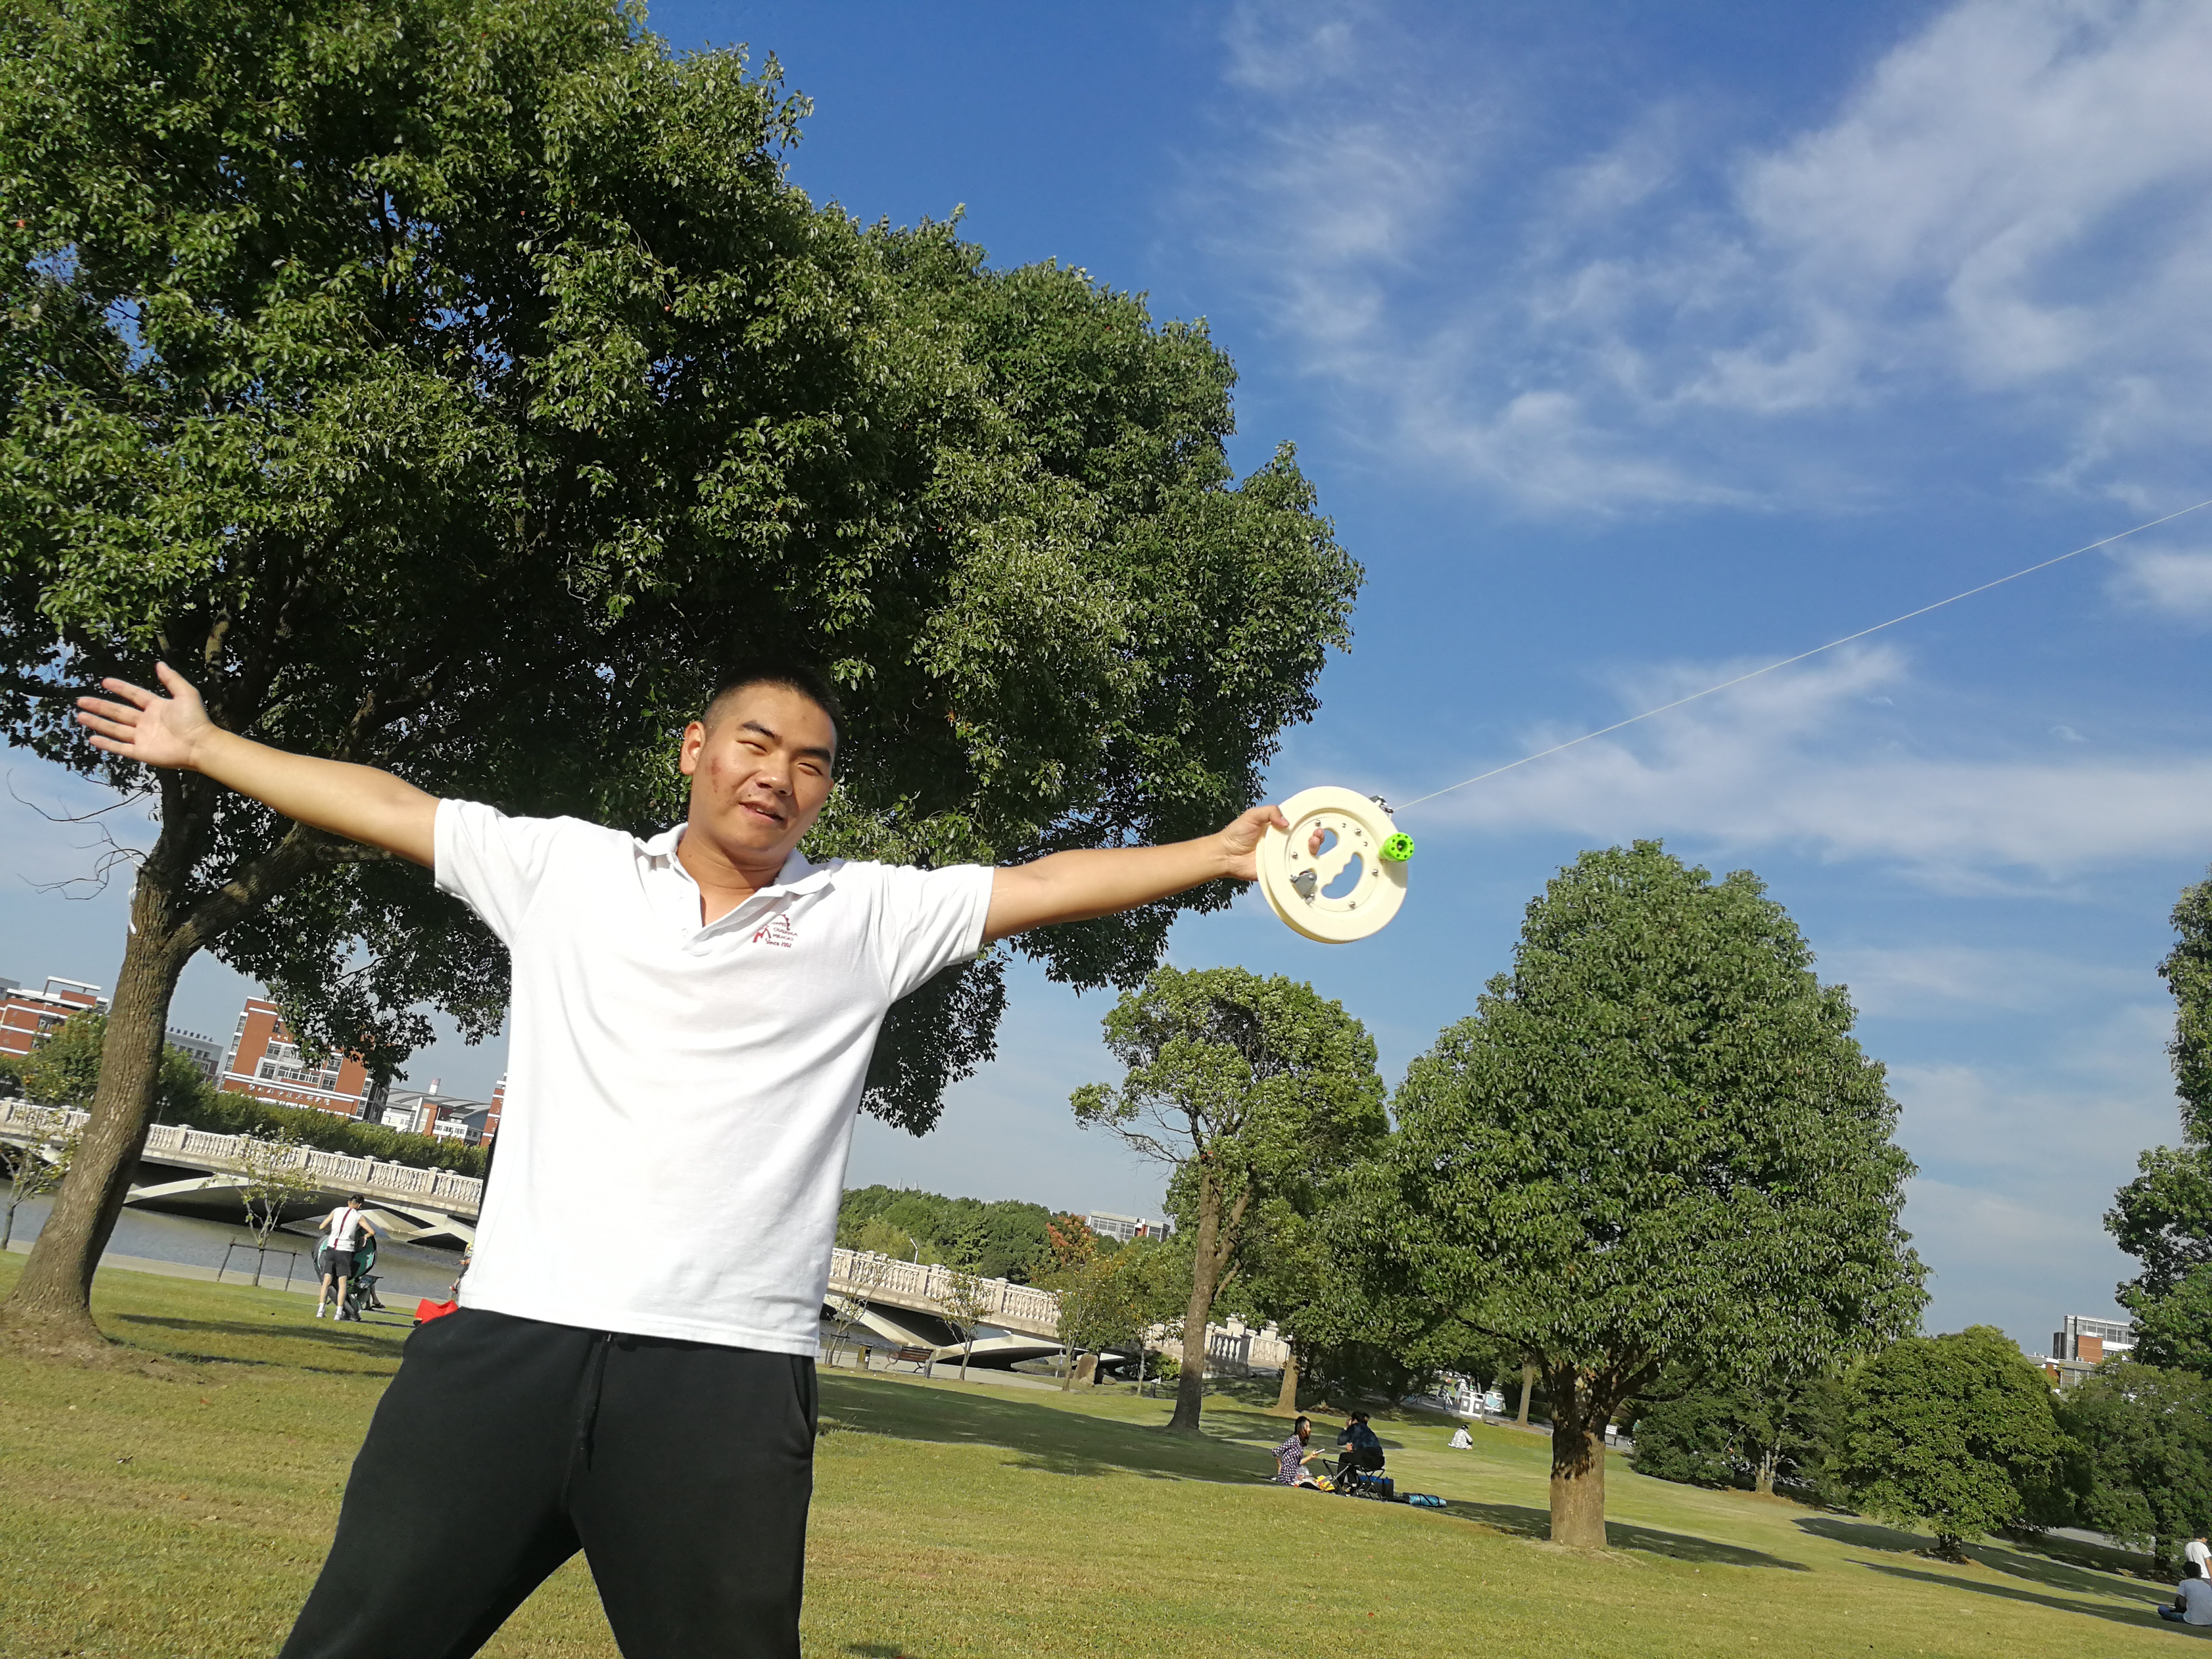
\includegraphics[scale=0.5]{pic.png}

\subsection*{build}
\includegraphics[scale=0.3]{28.png}


\subsection*{(2)}

\begin{table}
\centering
\begin{tabular}{lllllp{0.3\columnwidth}}
\toprule
rank & F-norm \\
\hline
1 & 97.3 \\
2 & 98.1  \\
4 & 98.8 \\
16 & 99.8 \\
\bottomrule
\end{tabular}
\caption{Feature id}
\label{tab:feature}
\end{table}










\section*{Exercise 3.32}

\subsection*{(1)}

\includegraphics{32.png}

\subsection*{(2)}

We can do this.

It is a almost 4-dimensional space and needed to truncked to 3-dimensional.
Determine how the quality of reconstruction 
varies when you reduce points to distances using different metrics.

\begin{lstlisting}
rng default   % Set the seed for reproducibility
A = [normrnd(0,1,10,3) normrnd(0,0.1,10,1)];
B = randn(4,4);
X = A*B;
D = pdist(X,'euclidean'); % distance
Y = cmdscale(D);
maxerr2 = max(abs(pdist(X)-pdist(Y(:,1:2)))) 
maxerr3 = max(abs(pdist(X)-pdist(Y(:,1:3)))) 
maxerr4 = max(abs(pdist(X)-pdist(Y)))

D = pdist(X,'cityblock');
[Y,e] = cmdscale(D);
maxerr = max(abs(pdist(X)-pdist(Y)))
\end{lstlisting}


\attachfile{code.py}

\end{document}
